\chapter{Verbindung}

\section{Sprachassistenten-Steuerung}

\section{Weboberfläche}

\section{RFID}

\section{Ultraschallsensor}
\section{Piezo-Lautsprecher}

\section{Steckplan}

Auf \ref{Steckplan} ist die schlussendlich verwendete Steckung abgebildet. Der dazugehörge Elektrische Schaltplan findet sich in Anlage X %TODO


\begin{figure}
	\centering 
	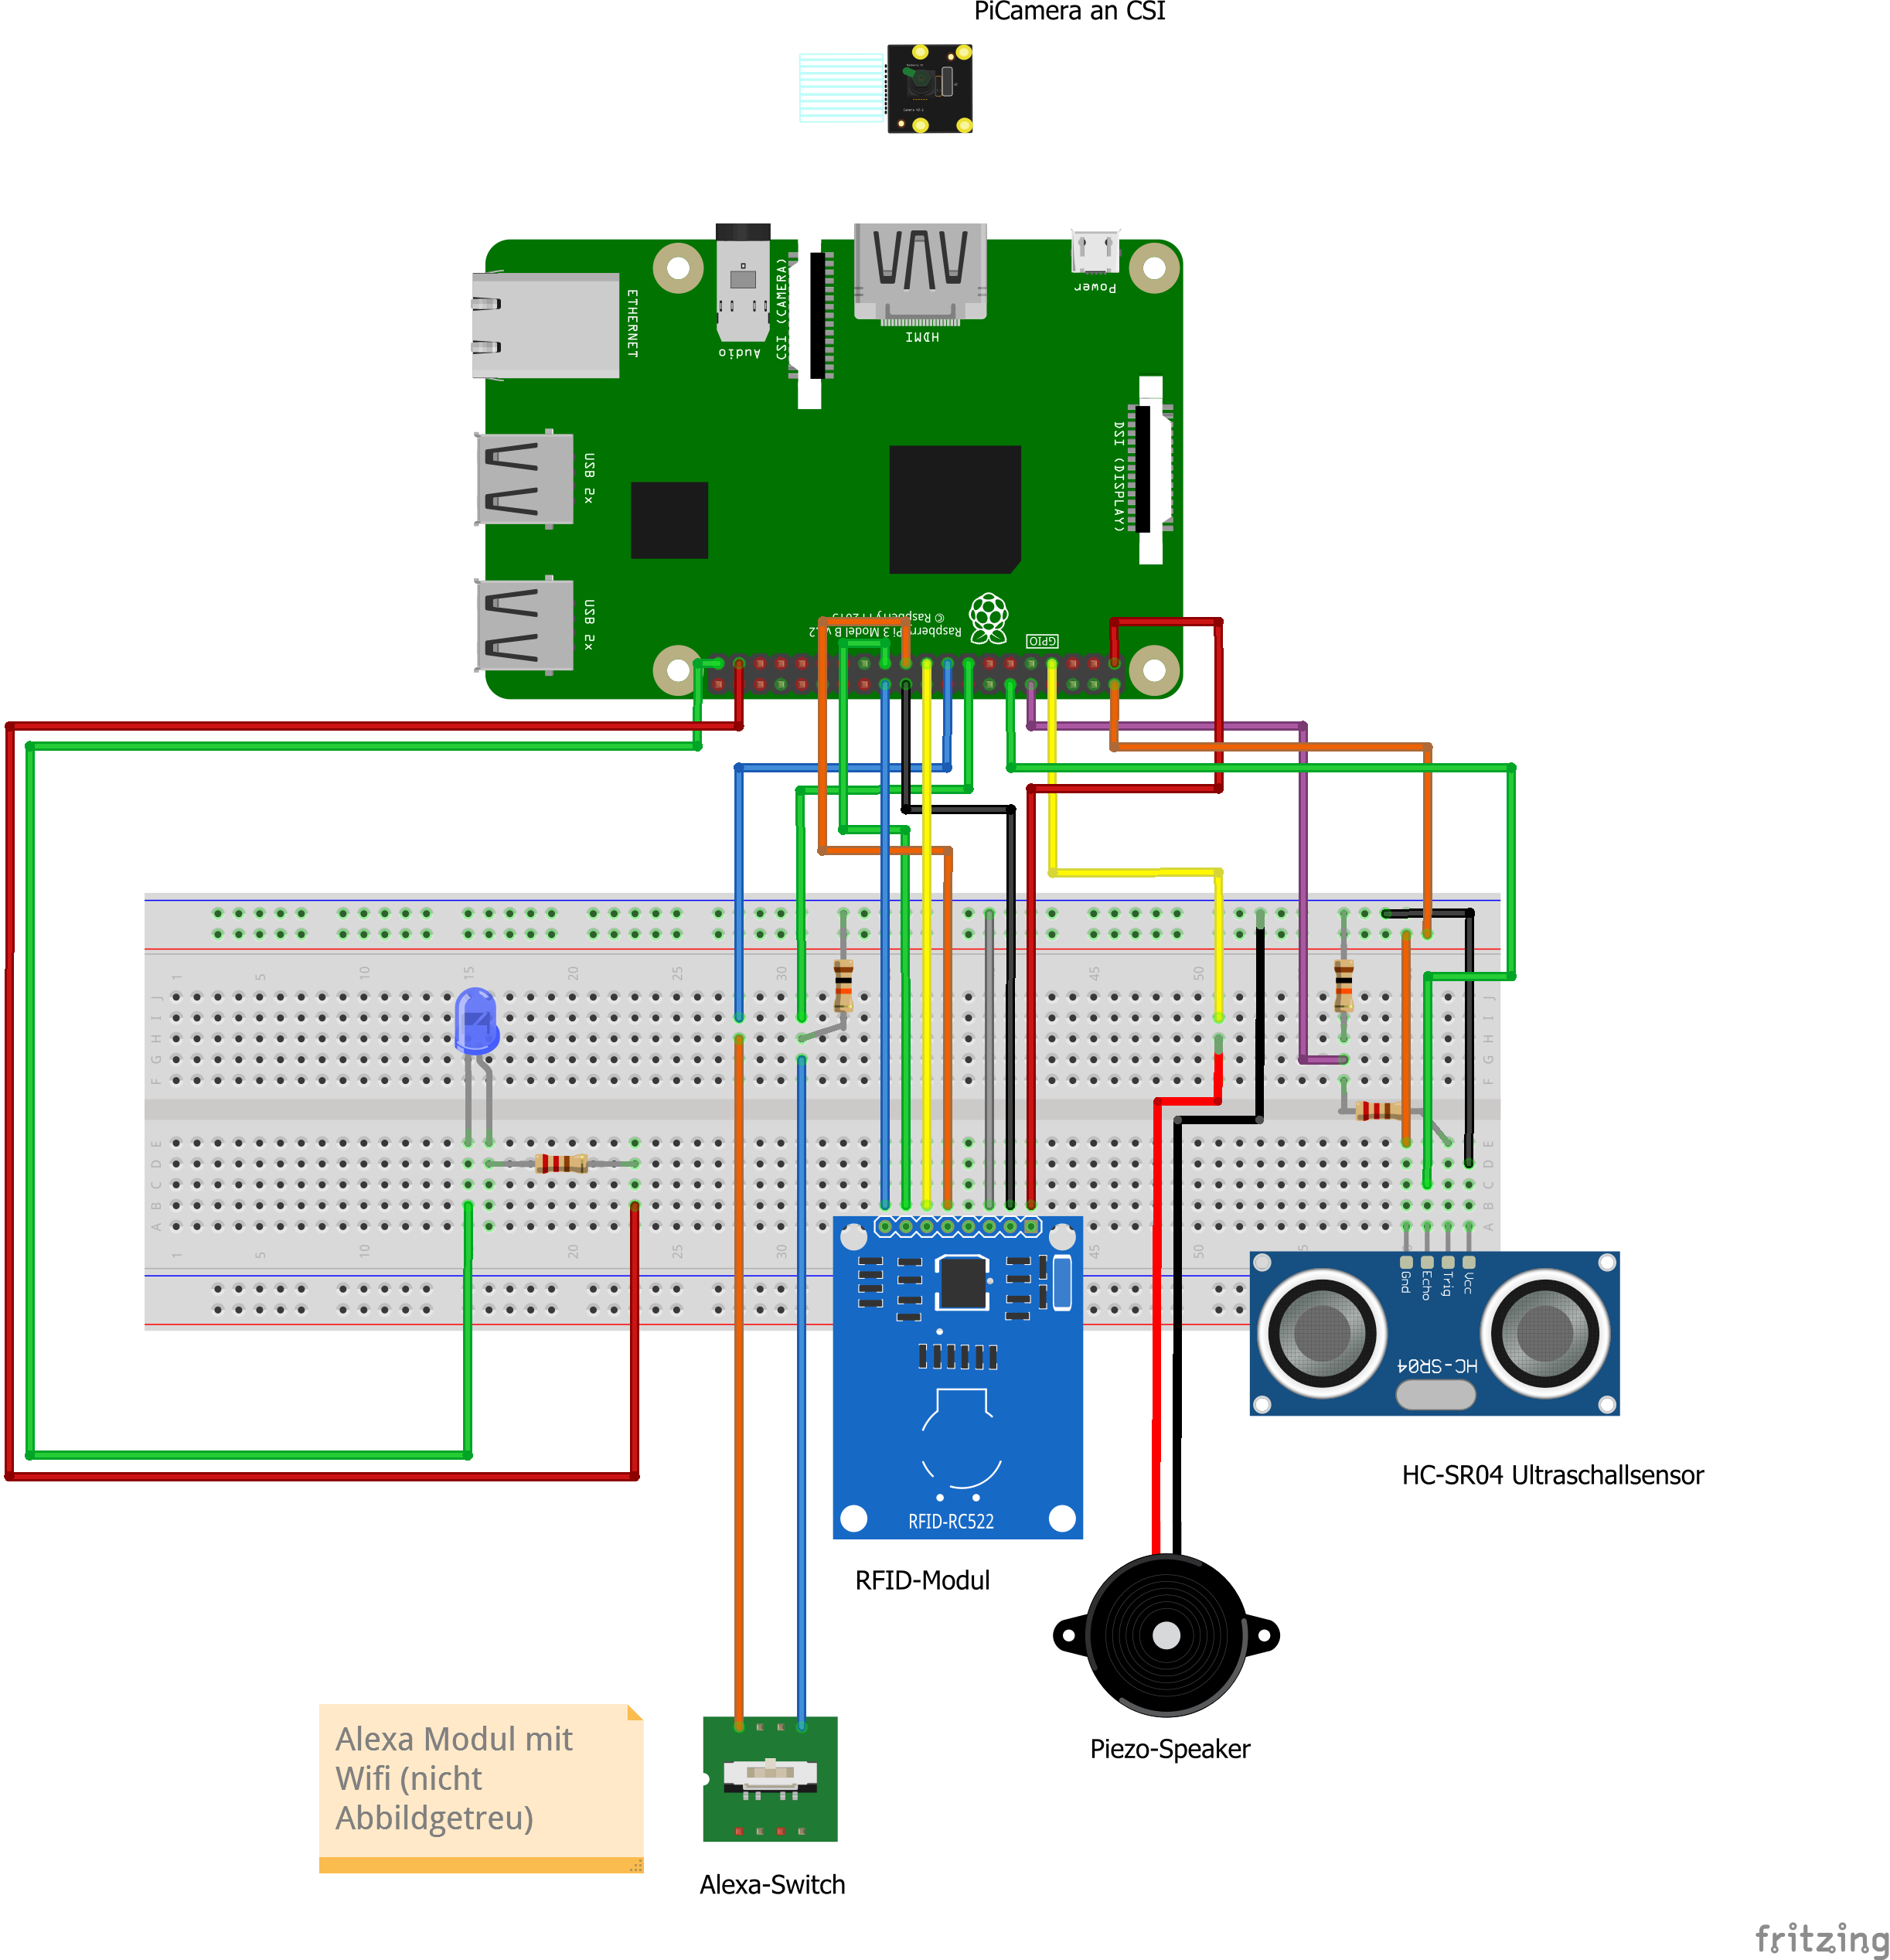
\includegraphics[scale=0.8]{\imagedir/SmartGarage.png}
	\captionsetup{format=hang}
	\caption[Steckplan]{\label{fig:test}Steckplan der gesamten Hardware \\Quelle: Eigene Darstellung}
\end{figure}






\section{Schaltlogik}

\begin{figure}
	\centering 
	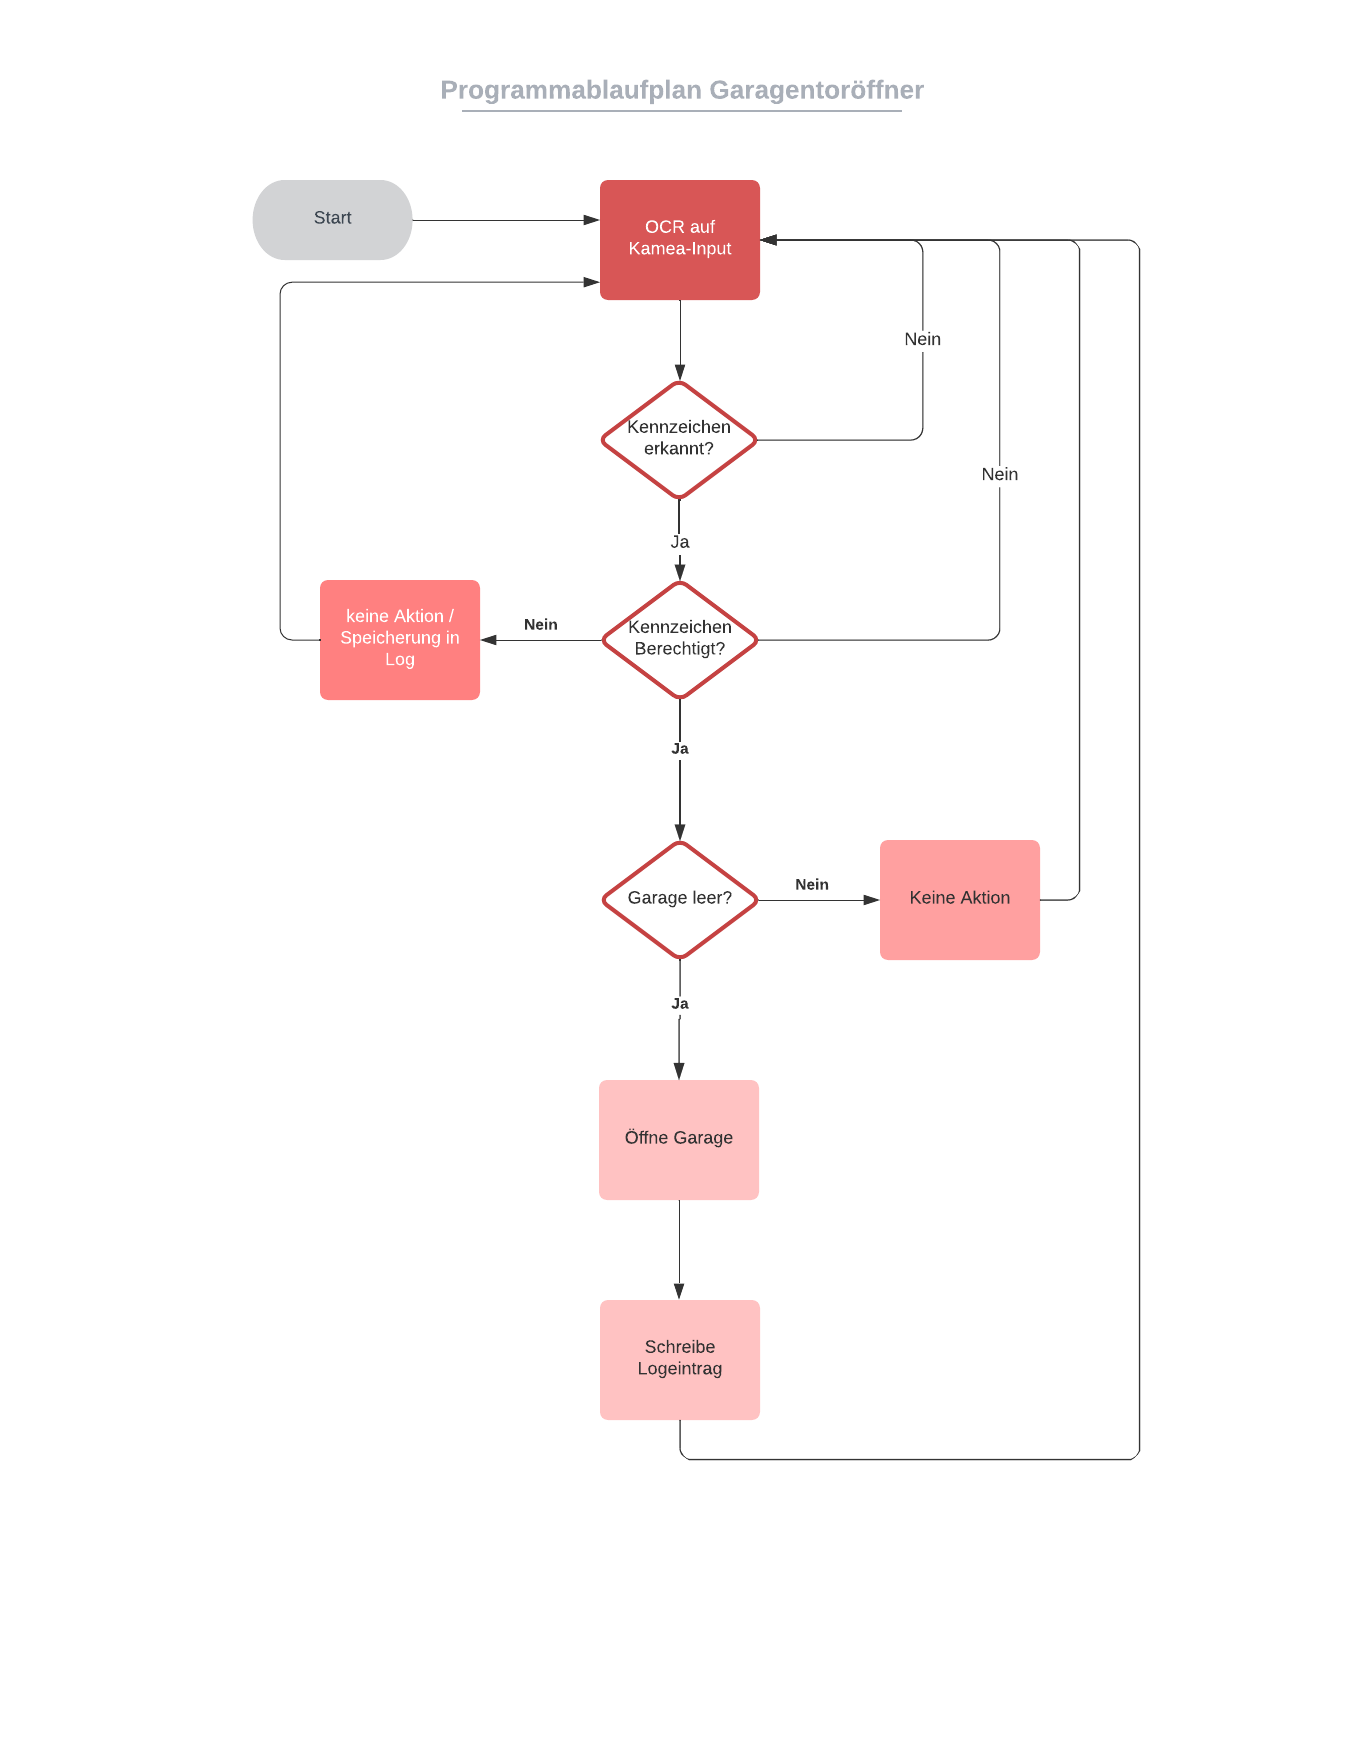
\includegraphics[scale=0.8]{\imagedir/Programmablaufplan.png}
	\captionsetup{format=hang}
	\caption[Programmablauf]{\label{fig:test}Ablauf der Kennzeichenerkennungs-Schleife \\Quelle: Eigene Darstellung}
\end{figure}



\section{Weboberfläche}




\chapter{Risiken und Limitierungen}

Mehrere problematische Punkte konnten innerhalb der relativ kurzen Projektlaufzeit noch nicht ausreichend adressiert werden. 

Zum einen hat die verwendete Software noch Schwierigkeiten mit Störungen durch Fahrzeug- und Kennzeichenhalterbeschriftungen und deutsche Umlaute, die in manchen Kennzeichen vorhanden sind, können noch nicht erkannt werden. Dies war auf den erfassten Testdaten in Mannheim/Heidelberg nicht nicht problematisch, wird es aber für andere Regionen sein.
Zum anderen ergeben sich natürlich durch die optische Erkennung etliche Probleme bei erschwerten Sichtverhältnissen wie Schnee, Regen, Dunkelheit oder schlicht verschmutzten Kennzeichen. 

Ein weiterer Bedeutender Punkt ist die mangelnde Sicherheit des Systems. Da die Öffnung des Garagentors nur durch das Kennzeichen geschieht, ist das Missbrauchs-Bzw. Einbruchspotenzial groß

\chapter{Wirtschaftliche Aspekte}

Auch wenn die technische Konzeption und Umsetzung im Mittelpunkt dieser Arbeit stehen, soll aufgrund der Ausrichtung des Studiengangs hier kurz auf einige Wirtschaftliche Aspekte eingegangen werden.
Entwicklungskosten \newline

3x Workshops a 12 Stunden
1x 24 Stunden 


Materialkosten%\footnote{Alle Preise in €, inkl. Versand}

\begin{tabular}[h]{lcr}
Raspberry Pi 3	&   39,95 \autocite{Pi3b} \newline \\
RFID-Modul RC552 &		5,00\autocite{RFID} \newline\\
Ultraschallmodul	&  8,94\autocite{SR04} \newline \\
Amazon Alexa Wifi Modul & 13,99\autocite{eWe}	\\
OAK-D Kamera & 185,51 \\
\textbf{Summe}			&	\textbf{253,39}
\end{tabular} \newline



Materialkosten je Einheit
Raspberry Pi 3 			   39,95
RFID-Modul RC552			5,00
Ultraschallmodul HC-SR04	4,99





